%%%%%%%%%%%%%%%%%%%%%%%%%%%%%%%%%%%%%%%%%
% Jacobs Portrait Poster
% LaTeX Template
% Version 1.0 (31/08/2015)
% (Based on Version 1.0 (29/03/13) of the landscape template
%
% Created by:
% Computational Physics and Biophysics Group, Jacobs University
% https://teamwork.jacobs-university.de:8443/confluence/display/CoPandBiG/LaTeX+Poster
% 
% Further modified by:
% Nathaniel Johnston (nathaniel@njohnston.ca)
%
% Portrait version by:
% John Hammersley
%
% The landscape version of this template was downloaded from:
% http://www.LaTeXTemplates.com
%
% License:
% CC BY-NC-SA 3.0 (http://creativecommons.org/licenses/by-nc-sa/3.0/)
%
%%%%%%%%%%%%%%%%%%%%%%%%%%%%%%%%%%%%%%%%%

%----------------------------------------------------------------------------------------
%	PACKAGES AND OTHER DOCUMENT CONFIGURATIONS
%----------------------------------------------------------------------------------------

\documentclass[final]{beamer}

\usepackage[scale=1]{beamerposter} % Use the beamerposter package for laying out the poster
\usepackage{xcolor}
\usepackage{amsmath}
\usepackage{amssymb}
\usepackage{siunitx}
\usepackage{braket}
\usepackage{bbold}
\usepackage{bigints}
\usepackage{mathtools}
\usepackage{bm}

\sisetup{detect-all,mode=math,math-rm=\mathrm}

\definecolor{ubcblue}{cmyk}{1,0.9,0.13,0.68}
\definecolor{ubcblue1}{cmyk}{1,0.68,0.04,0}
\definecolor{ubcblue2}{cmyk}{0.8,0.12,0.01,0}
\definecolor{ubcblue3}{cmyk}{0.64,0.1,0.01,0}
\definecolor{ubcblue4}{cmyk}{0.52,0.05,0.03,0}
\definecolor{ubcblue5}{cmyk}{0.38,0.02,0.05,0}

\usetheme{confposter} % Use the confposter theme supplied with this template

\setbeamercolor{block title}{fg=ubcblue,bg=white} % Colors of the block titles
\setbeamercolor{block body}{fg=black,bg=white} % Colors of the body of blocks
\setbeamercolor{block alerted title}{fg=white,bg=ubcblue} % Colors of the highlighted block titles
\setbeamercolor{block alerted body}{fg=black,bg=white} % Colors of the body of highlighted blocks
% Many more colors are available for use in beamerthemeconfposter.sty

%-----------------------------------------------------------
% Define the column widths and overall poster size
% To set effective sepwid, onecolwid and twocolwid values, first choose how many columns you want and how much separation you want between columns
% In this template, the separation width chosen is 0.024 of the paper width and a 4-column layout
% onecolwid should therefore be (1-(# of columns+1)*sepwid)/# of columns e.g. (1-(4+1)*0.024)/4 = 0.22
% Set twocolwid to be (2*onecolwid)+sepwid = 0.464
% Set threecolwid to be (3*onecolwid)+2*sepwid = 0.708

\newlength{\sepwid}
\newlength{\onecolwid}
\newlength{\twocolwid}
\newlength{\threecolwid}
\setlength{\paperwidth}{36in} % A0 width: 46.8in
\setlength{\paperheight}{48in} % A0 height: 33.1in
\setlength{\sepwid}{0.024\paperwidth} % Separation width (white space) between columns
%\setlength{\onecolwid}{0.22\paperwidth} % Width of one column
%\setlength{\twocolwid}{0.464\paperwidth} % Width of two columns
%\setlength{\threecolwid}{0.708\paperwidth} % Width of three columns
\setlength{\onecolwid}{0.3013\paperwidth} % Width of one column
\setlength{\twocolwid}{0.6267\paperwidth} % Width of two columns
\setlength{\topmargin}{-0.5in} % Reduce the top margin size
%-----------------------------------------------------------

\usepackage{graphicx}  % Required for including images

\usepackage{booktabs} % Top and bottom rules for tables
\usepackage{eso-pic}

%----------------------------------------------------------------------------------------
%	TITLE SECTION 
%----------------------------------------------------------------------------------------

\title{Incoherent tunneling and topological \\superconductivity in twisted cuprate bilayers}

\author{\underline{Rafael Haenel}\inst{1,2}, Tarun Tummuru\inst{1,3}, Marcel
Franz\inst{1}}

\institute{
	\inst{1} Department of Physics and Astronomy \& Stewart Blusson Quantum
	Matter Institute, University of British Columbia \\
	\inst{2} Max Planck Institute for Solid State Research \quad
\inst{3} Department of Physics, University of Zurich}
%----------------------------------------------------------------------------------------

\usepackage{exscale}
\begin{document}

\newcommand\AtPagemyLowerLeft[1]{\AtPageLowerLeft{%
\put(\LenToUnit{0.805\paperwidth},\LenToUnit{0.957\paperheight}){#1}}}
\newcommand\AtPagemyLowerRight[1]{\AtPageLowerLeft{%
\put(\LenToUnit{0.014\paperwidth},\LenToUnit{0.953\paperheight}){#1}}}
\AddToShipoutPictureFG{
  \AtPagemyLowerLeft{{
\includegraphics[width=17cm,keepaspectratio]{fig/logos3}}}
}%
\AddToShipoutPictureFG{
	\AtPagemyLowerRight{{
\includegraphics[width=10.5cm,keepaspectratio]{fig/ubc_qmi}}}
}%


\addtobeamertemplate{block end}{}{\vspace*{2ex}} % White space under blocks
\addtobeamertemplate{block alerted end}{}{\vspace*{2ex}} % White space under highlighted (alert) blocks

\setlength{\belowcaptionskip}{2ex} % White space under figures
\setlength\belowdisplayshortskip{2ex} % White space under equations

\begin{frame}[t] % The whole poster is enclosed in one beamer frame

\begin{columns}[t] % The whole poster consists of three major columns, the second of which is split into two columns twice - the [t] option aligns each column's content to the top

\begin{column}{\sepwid}\end{column} % Empty spacer column

\begin{column}{\onecolwid} % The first column

%----------------------------------------------------------------------------------------
%	OBJECTIVES
%----------------------------------------------------------------------------------------

\begin{alertblock}{Summary}
We report the observation of a large ZBCP in superconducting junction structures mediated by 
surface states of the Dirac semimetal Cd$_3$As$_2$. Our detailed analyses
suggest that this large ZBCP is most likely not caused by MZMs. We attribute it,
instead, to the existence of a supercurrent between two far-separated
superconducting Al electrodes.
\end{alertblock}

%----------------------------------------------------------------------------------------
%	INTRODUCTION
%----------------------------------------------------------------------------------------

\begin{block}{Introduction}



\begin{figure}
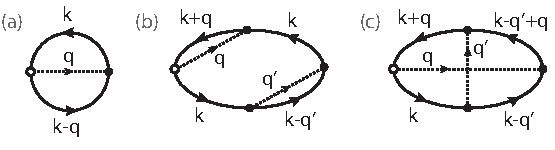
\includegraphics[width=\linewidth]{fig/diagram-figure.pdf}
\caption{\sffamily \, Device geometry and temperature and magnetic field dependence
	of differential conductance measured across the rightmost junction.}
\label{fig:exp}
\end{figure}

\begin{figure}[t]
	\centering
	\includegraphics[width=\columnwidth]{fig/phase-diagram.pdf}
	\caption{Phase diagram of incoherently coupled twisted bilayer cuprates. For a given $\Lambda$, the inside of the cone-shaped region breaks $\mathcal{T}$. Black-dashed lines mark the phase boundary in the clean limit, previously introduced in \cite{Can2021}. For increasing degree of momentum non-conservation $\Lambda$, the $\mathcal{T}$-breaking phase boundaries shrink towards $45^\circ$.}
	\label{fig:phasediagram}
\end{figure}
\begin{figure}[t]
	\centering
	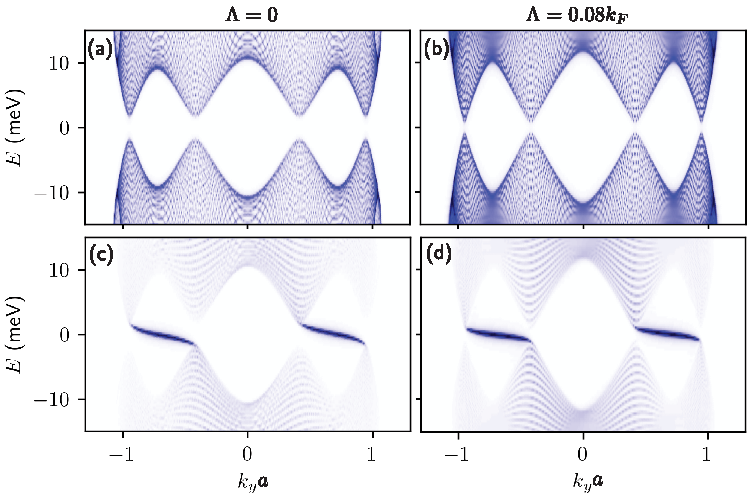
\includegraphics[width=\columnwidth]{fig/spectrum.pdf}
	\caption{Bulk (a-b) and boundary (c-d) spectrum for incoherently coupled cuprate bilayers with $\Lambda=0$ (left) and $\Lambda/k_F=0.08$ (right) at $45^\circ$ twist angle. The spectrum shows chiral edge modes traversing the bulk gap which is reduced but finite for increased $\Lambda$. Edge modes, which are in fact degenerate, indicate a Chern number $\mathcal{C}=4$. }
	\label{fig:edgemode}
\end{figure}


\end{block}
%----------------------------------------------------------------------------------------


\begin{block}{Model}


\end{block}

\end{column} % End of the first column


\begin{column}{\sepwid}\end{column} % Empty spacer column

\begin{column}{\onecolwid} % Begin a column (column 2)
\rmfamily
\justify
Column without block
\begin{block}{Majorana zero modes}



\end{block}

\begin{block}{ZBCP due to supercurrent}
\end{block}



\end{column} % End of the second column

\begin{column}{\sepwid}\end{column} % Empty spacer column

\begin{column}{\onecolwid} % The third column




\begin{block}{Magnetic field dependence}
\end{block}

%----------------------------------------------------------------------------------------
%	CONCLUSION
%----------------------------------------------------------------------------------------
\begin{block}{Conclusion}
Conclusion
\end{block}



%----------------------------------------------------------------------------------------
%	REFERENCES
%----------------------------------------------------------------------------------------

\begin{block}{References}

\nocite{*} % Insert publications even if they are not cited in the poster
\small{\bibliographystyle{unsrt}
\bibliography{lit}\vspace{0.75in}}

\end{block}


%----------------------------------------------------------------------------------------

\end{column} % End of the third column

\end{columns} % End of all the columns in the poster

\end{frame} % End of the enclosing frame

\end{document}
